% ----------------------------------------------------------------------
\section{Case study: PDPA}\label{sec:case_study_pdpa}

Singapore's Personal Data Protection Act \cite{pdpa_link} consists of a set of
rules governing the use of personal data in private and public organizations,
and describes actions to be taken if a data breach is detected. It consists on
the one hand of \emph{constitutive} rules, \ie{} definitions specifying
what is considered a data breach and under which conditions it is deemed a
notifiable data breach. On the other hand, \emph{regulative} rules prescribe
which actions need to be taken if a notifiable data breach is detected.

The constitutive rules are sufficiently voluminous and complex to warrant the
development of an expert system assisting organizations in assessing whether a
data breach is notifiable. In the CCLAW project, we have developed such a
system, which is described \remms{elsewhere. Reference?}. The regulative rules
are seemingly less involved but sufficiently intricate that actors that
precisely follow the rules may wind up in a state where they have breached the
law. The complexity results from the interplay of temporal conditions that
remain implicit and that would have to be explicated to guarantee lawful
behavior.

We here give an abridged account of the relevant rules; for details, see
\S\S~26A to E of \cite{pdpa_link} that leads to and motivates our
formalization in \secref{sec:formal_analysis}. The PDPA identifies three
actors in a data breach scenario:
\begin{itemize}
\item the \emph{organization} in which a data breach has occurred;
\item the Personal Data Protection Commission (PDPC, henceforth only called
  the \emph{commission}), the governmental authority that has to be notified
  in case of a breach;
\item the \emph{individual} affected by a data breach. The abstraction of the
  multitude of affected individuals to a single entity is already done in the
  law text and seems appropriate as there is no interaction among the
  individuals. 
\end{itemize}

The temporal requirements are as follows:
\begin{itemize}
\item When a data breach is detected, the organization has up to thirty days to
  assess whether the data breach is notifiable; if it is not, no further
  action is required, and the process stops there. 
\item If the breach is notifiable, the organization is obliged to inform the
  commission within three days of having recognized the breach as notifiable.
\item If the breach is notifiable, any affected individual also has to be
  informed within the three day period.
\item The organization must not notify an affected individual if the
  commission so directs.
\end{itemize}

The inconsistency, that was in part revealed by the formalization and then
confirmed by model checking, arises from the lack of temporal coordination
between the action of informing the commission and the individual, and
possibly the interdiction by the commission to inform the individual.


%----------------------------------------------------------------------
\section{Formal Analysis}\label{sec:formal_analysis}

%......................................................................
\subsection{Formal model}\label{sec:formal_model}

We have carried out a formal analysis of this scenario with Timed Automata
(TA) in the Uppaal \cite{larsen1997uppaal} model checker. The global setup is
shown in \figref{fig:pdpa}. There are three interacting automata, one for each
of the above-mentioned actors. The states carry names (in mauve), the initial
states are marked with a double circle. The automata synchronize via messages
(in turquoise), where a send action is indicated by an exclamation and a
receive action by a question mark. Transitions may depend on Boolean
conditions (here: variables such as \texttt{isNotifiable}) and on temporal
conditions modeled with the aid of \emph{clocks}. In this example, there is
one clock, \texttt{cl}, that is zero in the initial state, and that is again
reset to zero in the transition from the state \texttt{breachDetected} to
\texttt{breachDeterminedNotifiable}.


\begin{figure}[htp]
\centering
\subfloat[Commission\label{fig:commission}]{%
  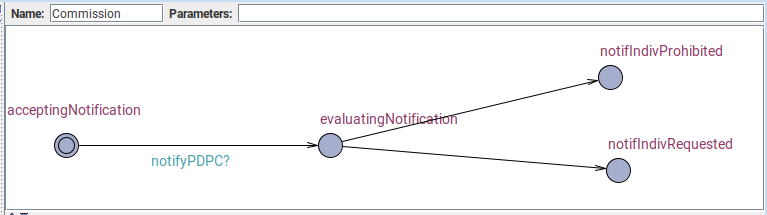
\includegraphics[width=0.65\textwidth]{Figures/commission.png}%
}\hfil
\subfloat[Individual\label{fig:individual}]{%
  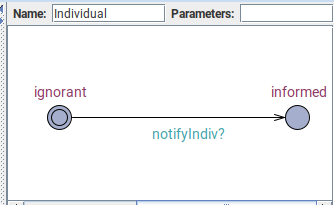
\includegraphics[width=0.3\textwidth]{Figures/individual.png}%
}\\
\subfloat[Organization\label{fig:organization}]{%
  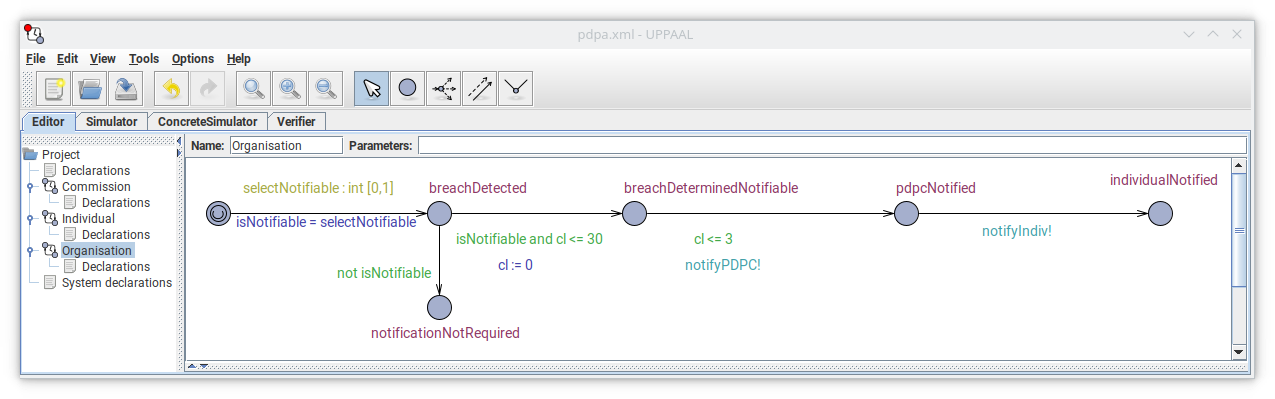
\includegraphics[width=\textwidth]{Figures/organization.png}%
}
\caption{Automata modeling the PDPA scenario}\label{fig:pdpa}
\end{figure}

According to the TA semantics, there are two kinds of transitions: the passage
of time, at the same rate in all automata, or discrete state changes along
enabled transitions, \ie{} transitions whose conditions are satisfied. In case
several transitions are enabled, one of them is chosen
non-deterministically. This happens for example in the Commission automaton
after receiving a notification (\texttt{notifyPDPC?}), modeling the fact that
the commission's decision to prohibit or request the notification of the
affected individual is autonomous and not influenced by external factors.
The Individual automaton only provides two states corresponding to whether the
individual has not yet / has been notified.

The Organization automaton is the
most complex one: the very first transition is a modeling artifact for giving
a random Boolean value to the variable \texttt{isNotifiable}. If the data
breach is not notifiable, the process ends. If the breach is determined to be
notifiable within 30 days, the timer is reset to allow for a 3 day period before
the notification is carried out. We have here made the choice to sequentialize
the notifications (the commission, then the individual). An interleaved execution
would be preferable but is hampered by limitations of Uppaal (no nested
parallel automata).

Let us note that our automaton model is not complete: not every execution of
the automata will run to completion, \ie{} wind up in one of the end nodes of
the automata. Instead, an execution can get stuck in an intermediate
state. This choice is deliberate, but open to debate: adding failure states
for every undesirable run would clutter up the automata; some runs may
legitimately be infinite without clearly identified end states; and, as seen
below, such deadlock states can be detected.

%......................................................................
\subsection{Checking the model}\label{sec:checking_the_model}

The model can be validated in several respects. The simplest form corresponds
to testing in traditional program development. For this, Uppaal (and similar
tools) provides a \emph{simulation} environment whose purpose is to step
through the model depending on user-selected criteria, for example the values
of Boolean variables or the duration of staying in particular sytsem
states. We will not further dwell on simulation, also because error traces
(see below) can be run in the simulator.

Contrasting with simulation is a systematic state space exploration by model
checking. Model checking can be used in legal drafting mode, to discover
incoherences in a law. It can also be used in ``production'' mode to identify
illegal behaviors and possible contrary-to-duty repair actions. We will
present examples of the two kinds below.

\begin{figure}[htp]
\centering
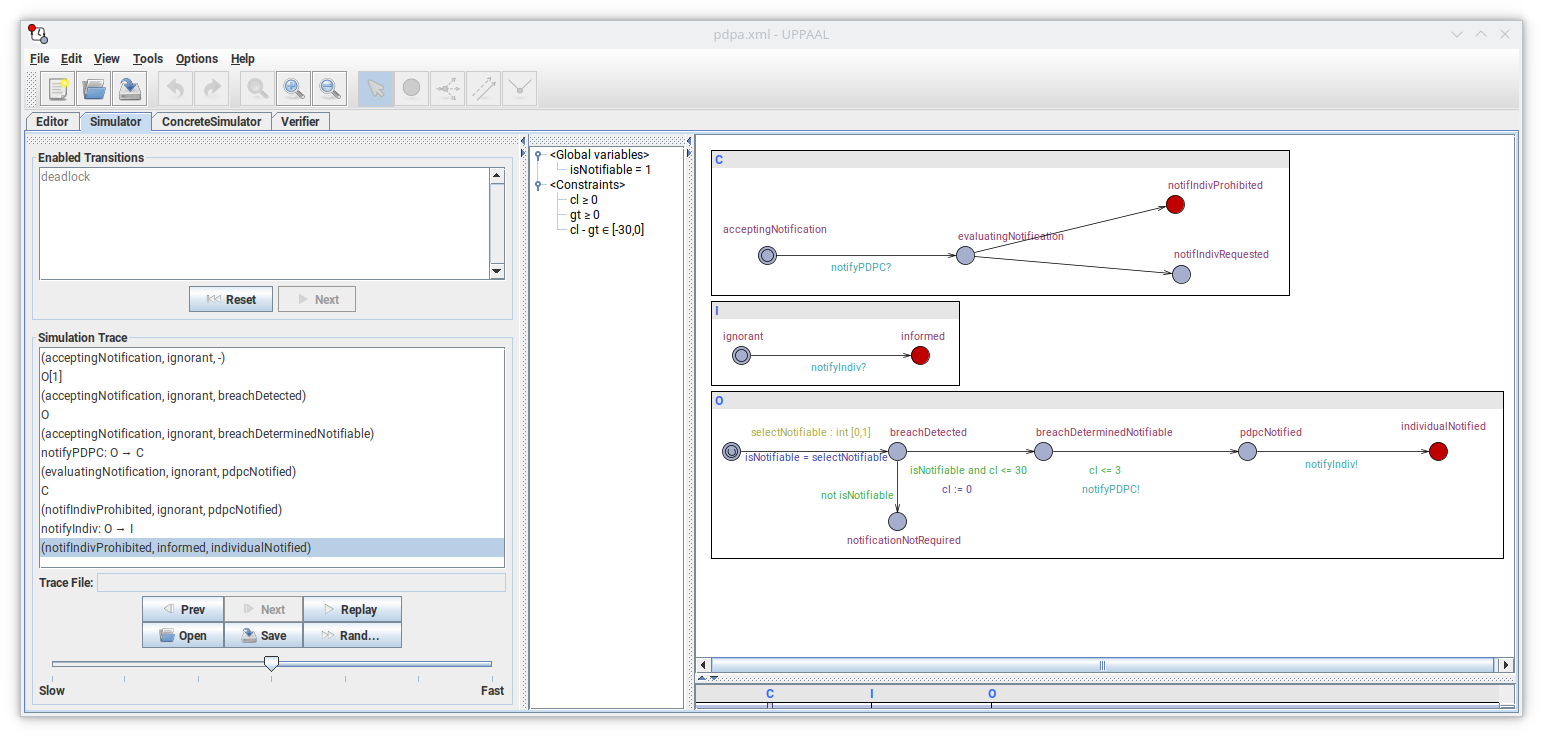
\includegraphics[width=\textwidth]{Figures/pdpa_trace.png}
\caption{Failure trace}\label{fig:pdpa_trace}
\end{figure}

Model checking tries to verify if a system's behavior conforms to requirements
that are typically stated in a formal logic, here the temporal logic CTL. We
give a few  examples in our scenario:

\begin{itemize}
\item A desirable property is that is possible to reach a state such that the
  individual is informed and the commission requests informing the
  individual. This property is written as \texttt{E<>I.informed and
    C.notifIndivRequested}. Here, \texttt{E<>} means: ``there exists a run
  eventually leading to''. and \texttt{I.informed} and
  \texttt{C.notifIndivRequested} refer to the corrosponding states in the
  Individual and Commmission automata. This property is indeed satisfied.

  
\item An undesirable situation is that the individual is informed in spite of
  the commission having prohibited it, expressed by the formula \texttt{E<>
    I.informed and C.notifIndivProhibited}. This property is also satisfied,
  and Uppaal produces a trace (\figref{fig:pdpa_trace}) leading to this error
  situation. It comes about because the organization has no clue at which
  point the commission's interdiction to inform the individual could
  intervene, and is therefore entitled to inform the individual as soon as a
  data breach is identified.

\item Another undesirable behavior is when the execution of the process gets
  stuck, or, more precisely, when there is a deadlock, in a system state that
  is not perceived as final. Note that in a technical sense, according to the
  terminology of labelled transition systems, every system with final states
  is deadlocked in these states. Identifying deadlocks in ``intermediate''
  states may contribute to finding leaks in the formal model, or states that
  correspond to breaches of the law. For example, the intermediate state
  \texttt{breachDeterminedNotifiable} is identified by the query \texttt{E<>
    O.breachDeterminedNotifiable and deadlock} as a deadlock state. Indeed, in
  this state, no action is possible when the notification deadline of 3 days
  has been exceeded.
\end{itemize}

%......................................................................
\subsection{Refinements}\label{sec:refinements}



\begin{itemize}
\item Introducing deadlines for feedback by the commission. If the feedback deadline is
  sufficiently close to the deadline for informing the individual, the law may
  not be formally inconsistent, but the process is not \emph{realizable} any
  more for a real organization. 
\end{itemize}

%----------------------------------------------------------------------
\section{Modularization}



%%% Local Variables:
%%% mode: latex
%%% TeX-master: "main"
%%% End:
